%!TEX root = ../thesis.tex
%*******************************************************************************
%*********************************** First Chapter *****************************
%*******************************************************************************

\chapter{Resistive Wall Simulation}  %Title of the First Chapter

\ifpdf
    \graphicspath{{Chapter8/Figs/Raster/}{Chapter8/Figs/PDF/}{Chapter8/Figs/}}
\else
    \graphicspath{{Chapter8/Figs/Vector/}{Chapter8/Figs/}}
\fi

\label{chapter 8}


%************************************************************************** 
\section{Validation Challenge}
We try to validate the resistive boundary condition we are using. However, in contemporary research, the validation of resistive wall models remains a challenging task. Several factors contribute to this challenge. Firstly, there are no experiments and standard tests cases for resistive wall simulations. In hydrodynamics, there are a lot of visualized experiments like shock diffractions done by Bryson \cite{bryson1961diffraction} and Schardin \cite{schardin1966stossrohre}. In MHD, there are several benchmark tests, such as Brio-Wu and Orszag-Tang rotor problem while most of them are remained numerically. Unlike the well-established scenarios in hydrodynamics, MHD often involve extreme conditions and complex effects \cite{pu2024unified} so that less experiments can be done and used in numerical validations. Among the existing benchmark tests, some, like the Brio-Wu test, are one-dimensional and cannot reflect the effects of a resistive wall, while others are not stable enough to be used for validating resistive walls. Additionally, even for a same test, the diversity in modeling approaches and purposes in different studies make it hard to have a standard result. Some may study the external kink instability and only model locally, like  Ghatak \textit{et al.} \cite{ghatak2007kink}. Some may use a resistive MHD model while we are using a ideal MHD model \cite{becerra2016resistive}. Due to these challenges, establishing a universally accepted validation method for resistive wall models is elusive. 

A cylindrical equilibrium test is employed by Ferraro \textit{et al.} \cite{ferraro2016multi} designed to model the resistive wall mode (RWM) within a simplified straight cylindrical geometry to compare the calculated linear growth rate against an analytic solution. This test serves as a benchmark, and has been utilized by researchers to validate their resistive MHD models with resistive walls \cite{becerra2016resistive,ferraro2016multi,chrysanthou2020}. In this work, an attempt is made to approximate their results using our ideal MHD model.

\section{Cylindrical Equilibrium}
The cylindrical equilibrium test is derived from Chrysanthou \cite{chrysanthou2020} with some initial data from Ferraro \textit{et al.} \cite{ferraro2016multi}. We conduct this simulation with Cartesian coordinate while the initial data is better described in cylindrical coordinates with $r$ and $\theta$ and a center at (0,0). In this test, the plasma is confined within a circle with a radius of 2. A contact discontinuity is set at $r=0.8825$, and the surrounding plasma is given an initial velocity directed towards the upper right. For the contact discontinuity, the $tanh$ functions are used in the initial configuration of the problem. $B_\theta$ is used to impose some perturbation, transformed in $B_x$ and $B_y$. These are given in the Table \ref{tab:cylindricalEquilibrium} and the demonstrating Plot in Figure \ref{fig:cylindricalEquilibriumInitial}. In this plot, the color box ranges are manually adjusted to make the features more obvious.
\begin{table}[H]
\centering
\caption{Initial data for cylindrical equilibrium.}
\begin{tabular}{|c|>{\centering\arraybackslash}m{10cm}|}
	\hline
	\textbf{States} & \textbf{Values} \\
	\hline
	\( \rho \) & \( 0.495 \cdot tanh[20\cdot(0.8825-r)]+0.505 \) \\
	\hline
	\( v_x \) & \( 10\cdot e^{-\frac{(0.8825-r)^2}{0.0625}} \) \\
	\hline
	\( v_y \) & \( 10\cdot e^{-\frac{(0.8825-r)^2}{0.0625}} \) \\
	\hline
	\( v_z \) & \( 0 \) \\
	\hline
	\( p \) & \( 0.45 \cdot tanh[20\cdot(0.8825-r)]+0.55 \) \\
	\hline
	\( B_r \) & \( 0 \) \\
	\hline
	\( B_{\theta} \) & \( \begin{cases}
		0.0815\cdot r/0.8825 & \text{if } r \leq 0.8825 \\
		0.0815\cdot0.8825/r & \text{if } r > 0.8825
	\end{cases} \) \\
	\hline
	\( B_z \) & \( 1.0 \) \\
	\hline
\end{tabular}
\label{tab:cylindricalEquilibrium}
\end{table}

\begin{figure}[H]
	\centering
	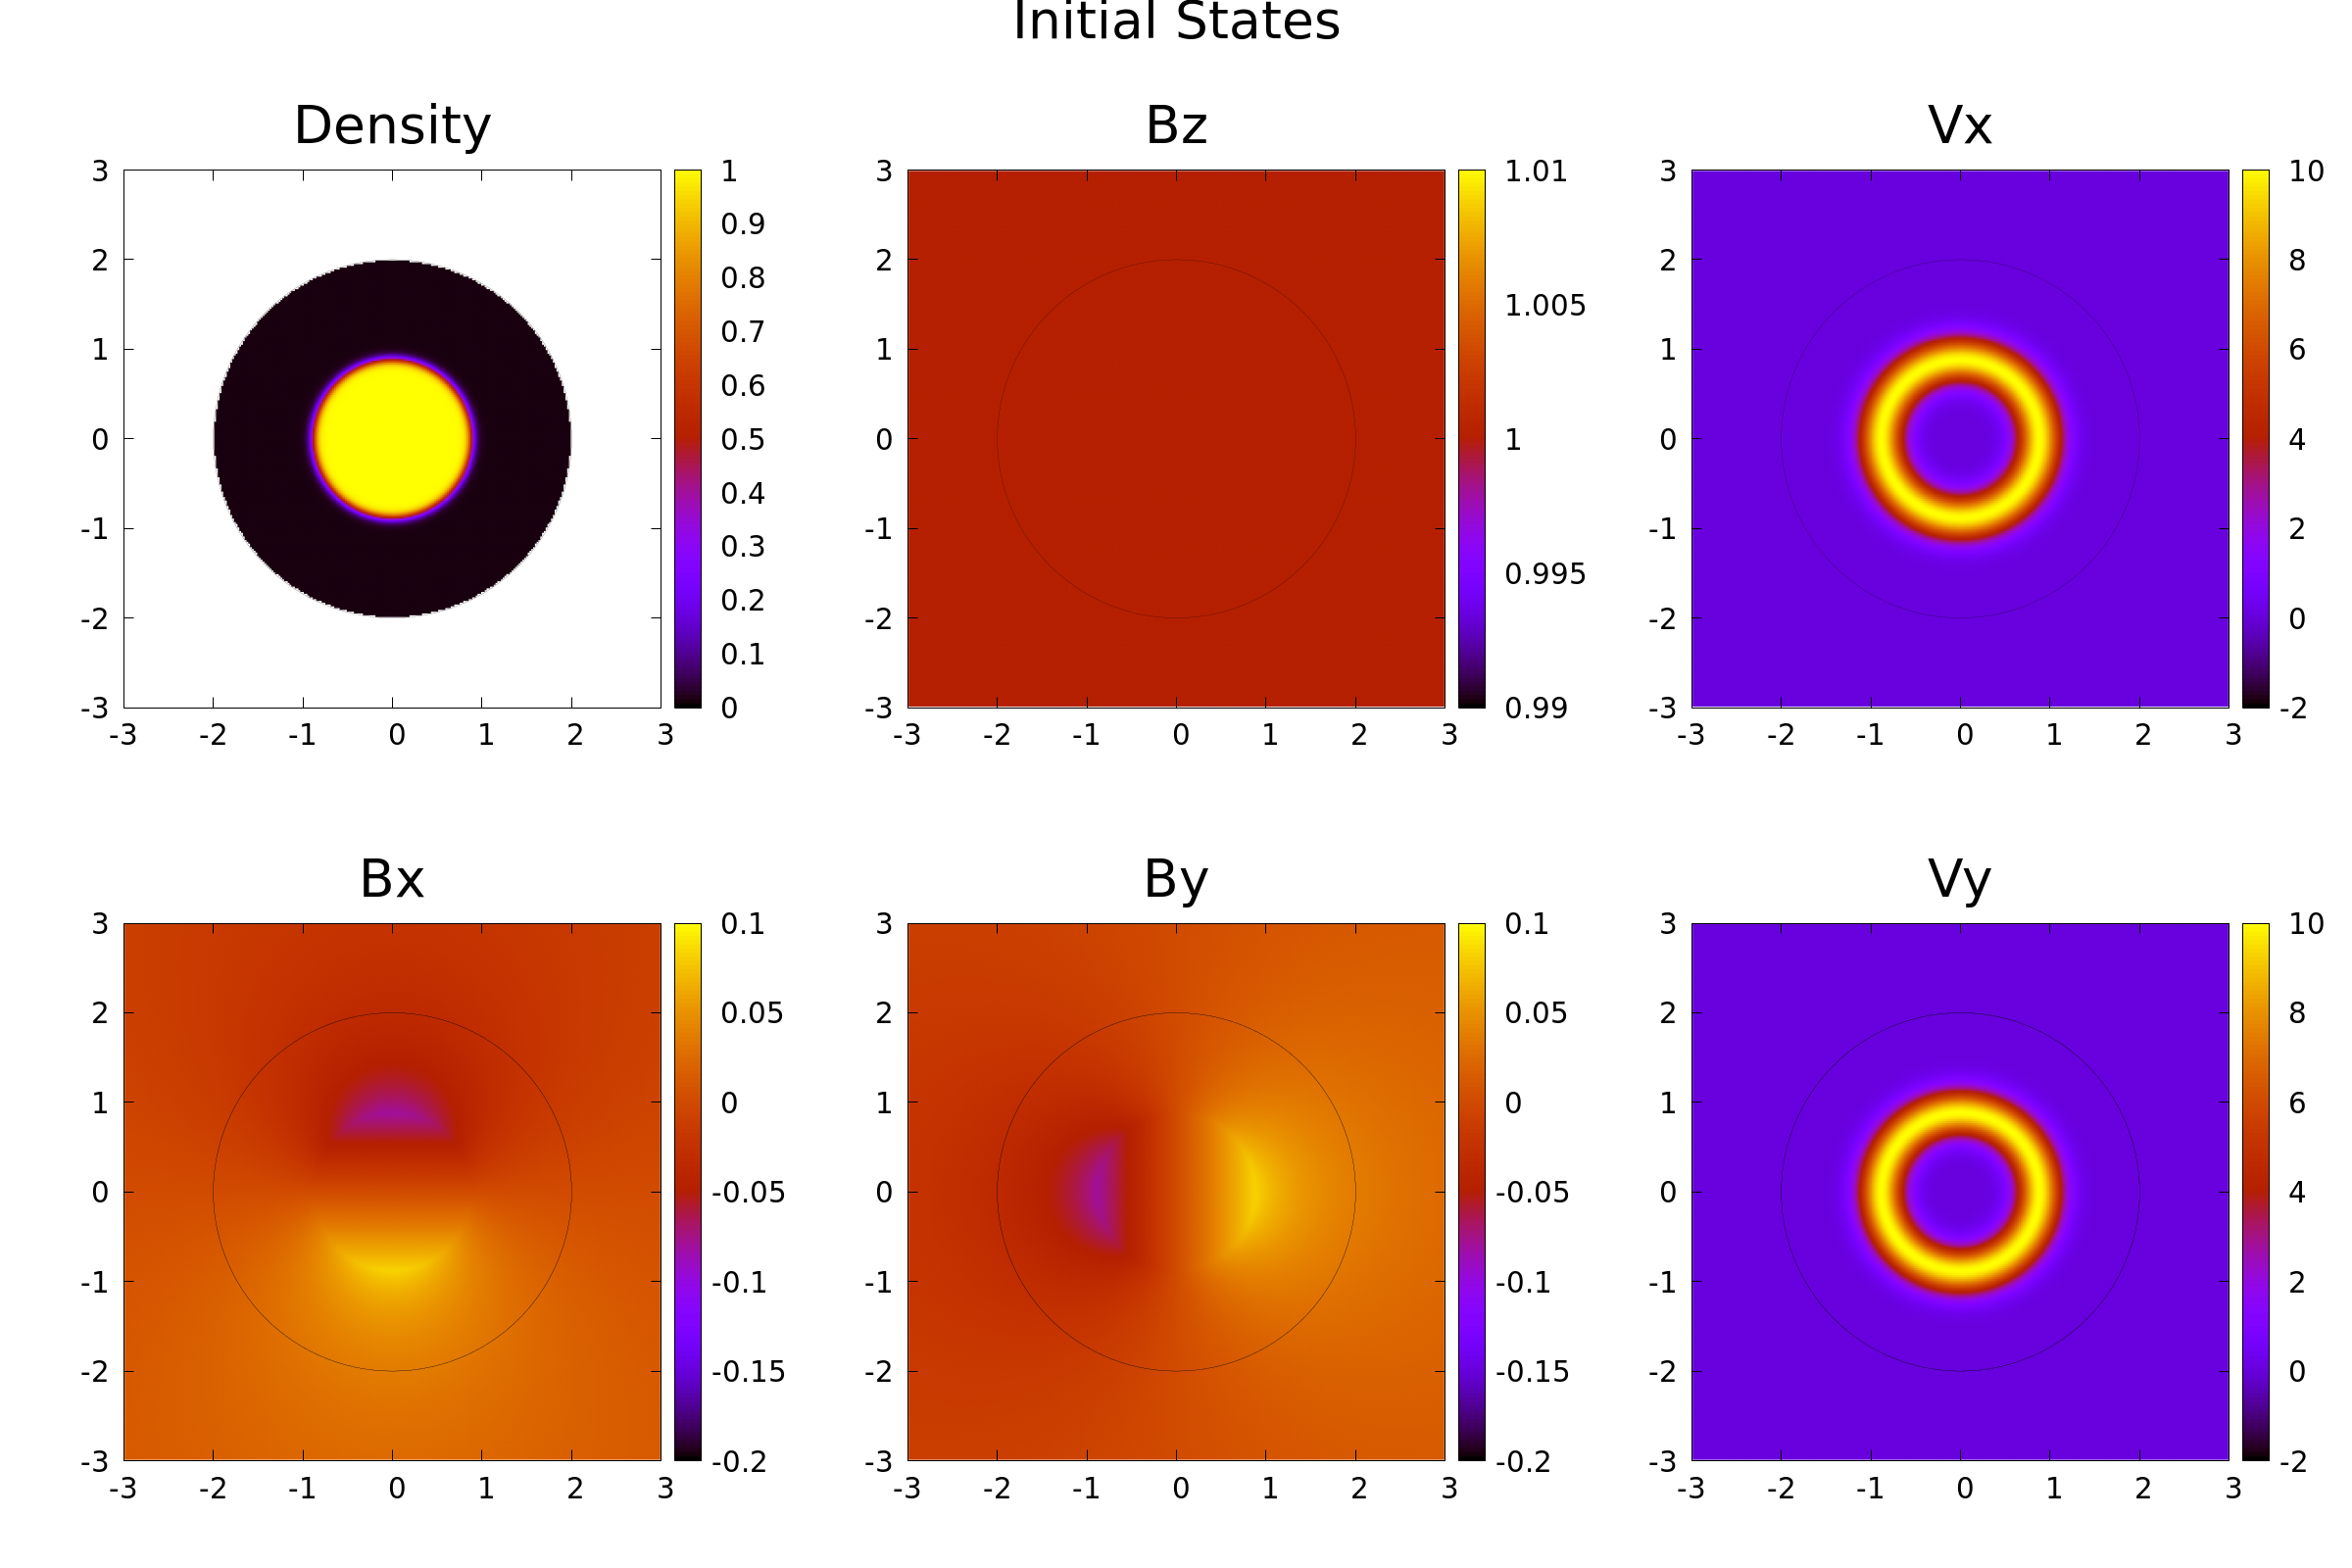
\includegraphics[width=1\linewidth]{InitialCylindricalEquilibrium.png}
	\caption[Initial states of cylindrical equilibrium]{Visualization of the initial states for cylindrical equilibrium. This test is built by Chrysanthou \cite{chrysanthou2020} based on some initial values from Ferraro \textit{et al.} \cite{ferraro2016multi}. The color box ranges are manually adjusted to make the features more obvious.}
	\label{fig:cylindricalEquilibriumInitial}
\end{figure}

After setting the initial states properly, the test is conducted within $300\times300$ resolution numerical area with $C_{CFL}=0.4$. Because of the possible stiffness of the resistive ODE, we use a low CFL number as an additional safety measure against numerical instabilities. The test is conducted to $t_{stop}=0.2$ after the core plasma hitting the boundary. Similar tests are conducted to make a comparison between perfect conducting condition $\eta_w=0.0$ and resistive condition $\eta_w=0.05$ as demonstrated in Figure \ref{fig:cylindricalEquilibrium}. 

The simulation results, depicted in Figure \ref{fig:cylindricalEquilibrium}, provide a comparison between the behavior of the system under perfect conducting walls (left column) and resistive walls with $\eta=0.05$ (right column). The two quantities examined are the plasma density (top row) and the magnetic field component $B_z$ (bottom row). While the overall behavior of the plasma appears similar across both boundary conditions, a notable difference emerges in the $B_z$ component. Under resistive conditions, the interaction between the plasma and the magnetic field within the rigid body leads to a significant increase in $B_z$.  This interaction causes the peak $B_z$ value within the plasma from 3.1758 in perfect conducting case to rise to 5.2921 in resistive case. On the other hand, changes in the plasma density are subtler, with only a slight increase in the peak density under resistive conditions, likely as a consequence of the magnetic field. In general, our result are in close qualitative agreement with Chrysanthou's results \cite{chrysanthou2020}.

\begin{figure}[H]
	\centering
	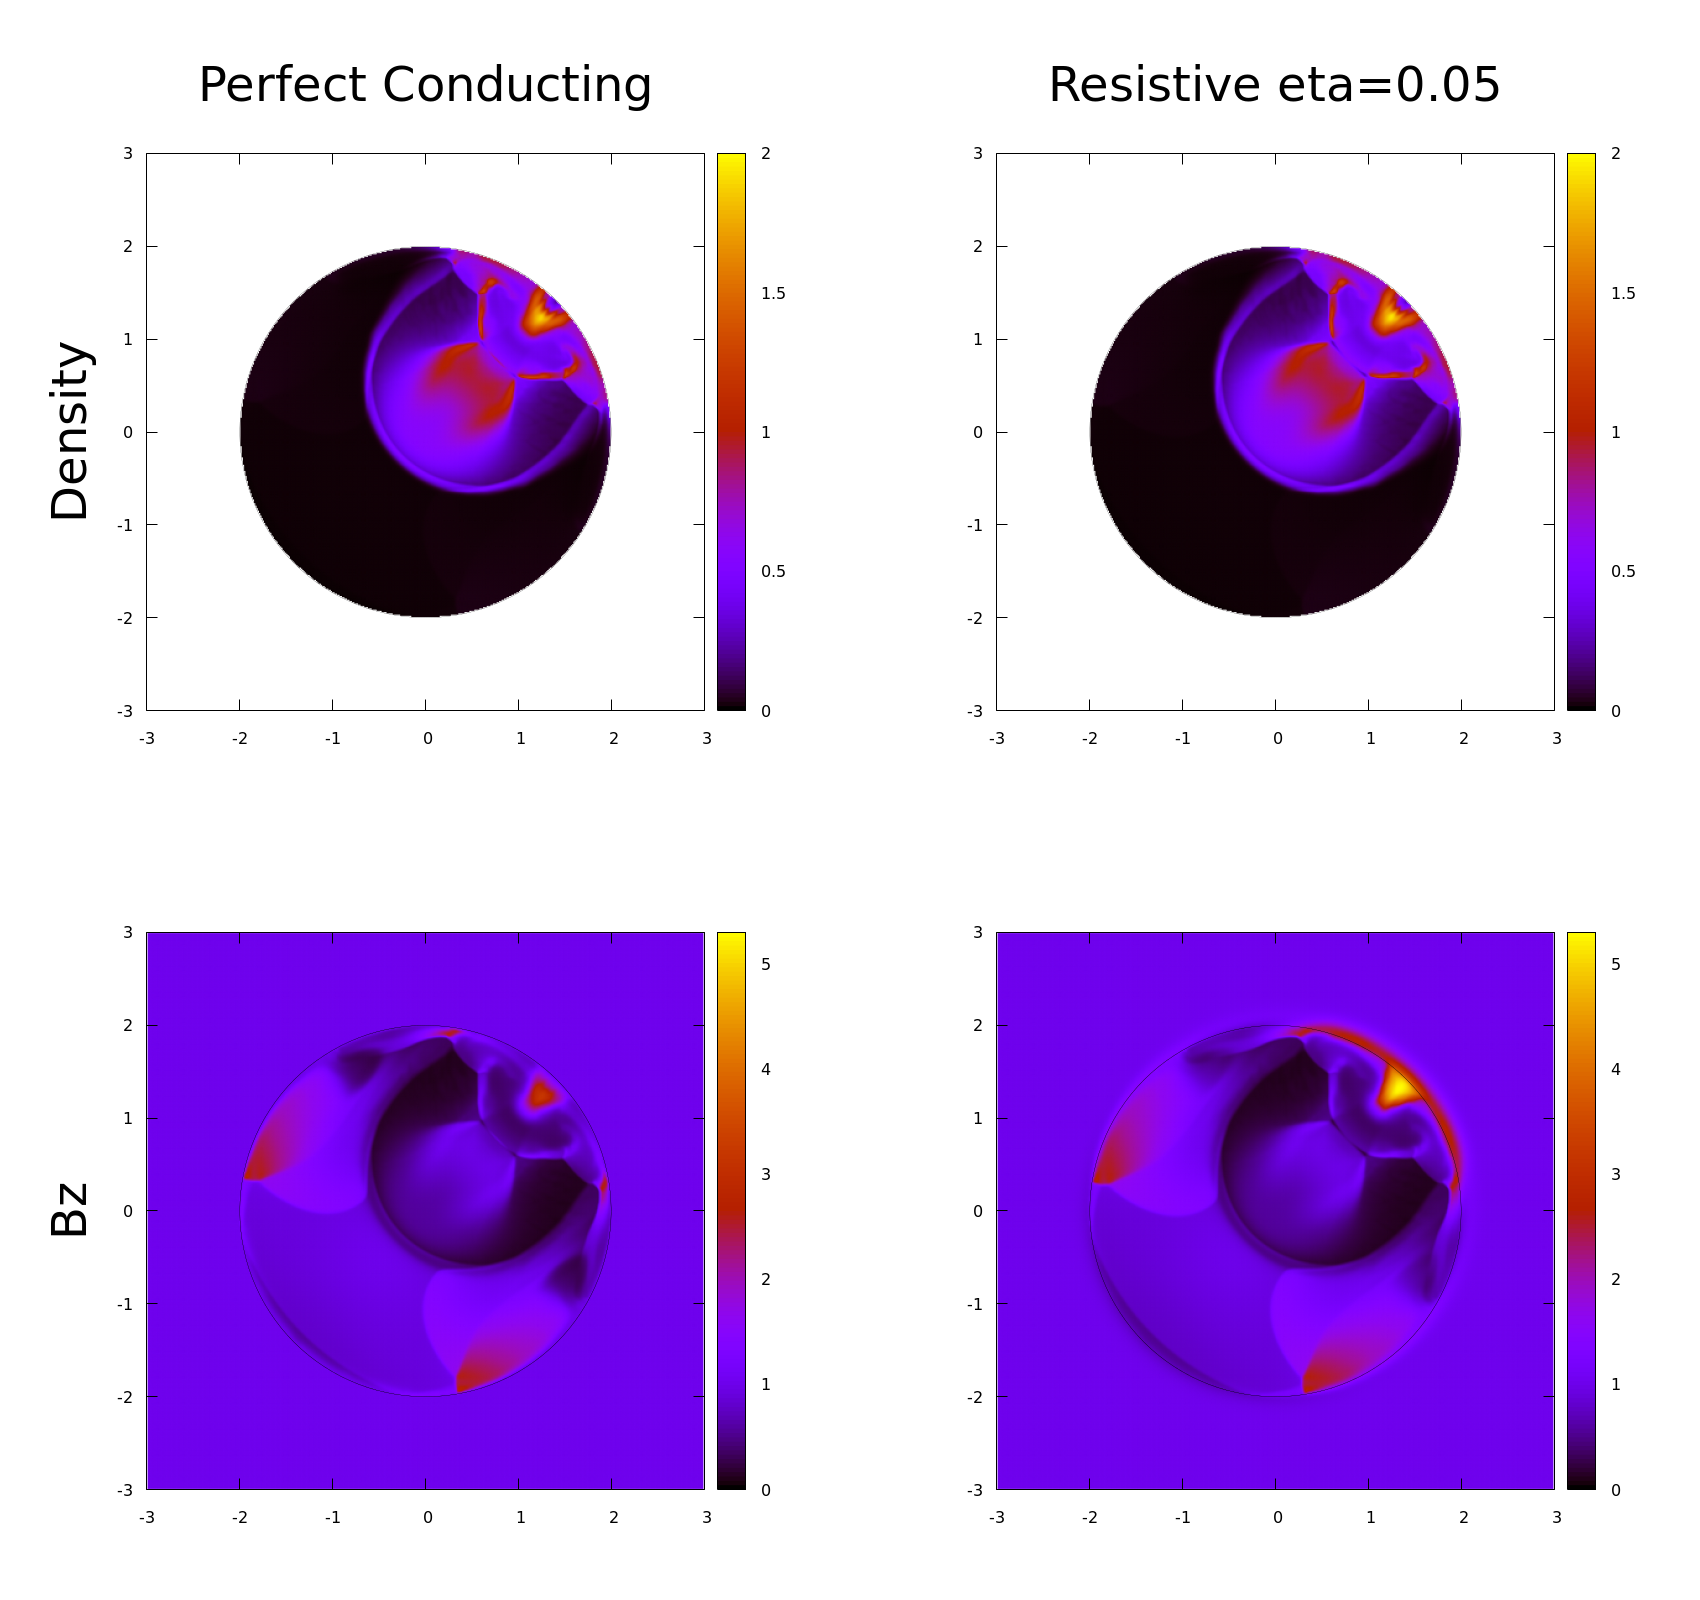
\includegraphics[width=1\linewidth]{cylindricalEquilibrium.png}
	\caption[Result of cylindrical equilibrium]{Results of the cylindrical equilibrium simulation. These plots compare the outcomes between a perfect conducting wall (left column) and a resistive wall $\eta=0.05$ (right column) with two key quantities, the plasma density (top row) and the magnetic field component $B_z$ (bottom row). Generally, they are similar in different boundary conditions. The primary difference is observed in the $B_z$ component. In the resistive scenario, the $B_z$ within the rigid body is significantly influenced by the plasma, leading to a noticeable increase. As a result, the peak $B_z$ value inside the plasma reaches 5.2921, compared to the 3.1758 peak in the perfect conducting case. However, the difference is hard to tell in density, except for a slight increase in the resistive density peak, which may be attributed to the influence of the magnetic field.}
	\label{fig:cylindricalEquilibrium}
\end{figure}

\subsubsection*{Total Energy}
Under ideal conditions, a perfect conducting wall should theoretically maintain a constant energy level within the system. However, the application of numerical methods such as the ghost fluid method can often lead to fluctuations or even reductions in total energy. When a resistive boundary condition is employed, the increase in resistivity allows more of the magnetic field to penetrate into the rigid body from the plasma. Consequently, the total energy within the plasma is expected to gradually decrease. To validate these hypotheses, we conducted a series of simulations. We accumulate the total energy over the whole plasma region and plot their curve as a function of time. The Figure \ref{fig:totalEnergy} below demonstrate temporal evolution of total energy. When $\eta_w=0.0$, the boundary condition used is the perfect conducting condition introduced in \ref{chapter 2}, the same as in the rotated Brio-Wu test; for $\eta_w>0.0$, the boundary condition is implemented by using the $\mathbf{B}$ values in the wall as ghost cells for the plasma, and vice versa, following the principles on wall outlined in equation \ref{equ:magneticDiffusion}. Overall, all the curves exhibit a downward trend. This may be attributed to the application of the ghost fluid method and the meshing revolution. As we incrementally increase $\eta_w$, the total final energy decreases, which aligns with our expectation that a more resistive wall allows greater magnetic field penetration, thereby reducing the total energy within the plasma. Furthermore, this decline appears to follow an exponential pattern. Although $\eta_w$ increases in fixed steps, the resulting decrease in total energy becomes progressively smaller. Notably, the gap between the curves for $\eta_w=0.0$ and $\eta_w=0.001$ is relatively large, potentially indicating the presence of some nonlinear behavior. This inconsistency will be discussed further in Chapter \ref{chapter 10}.

\begin{figure}[H]
	\centering
	\vspace{5mm}
	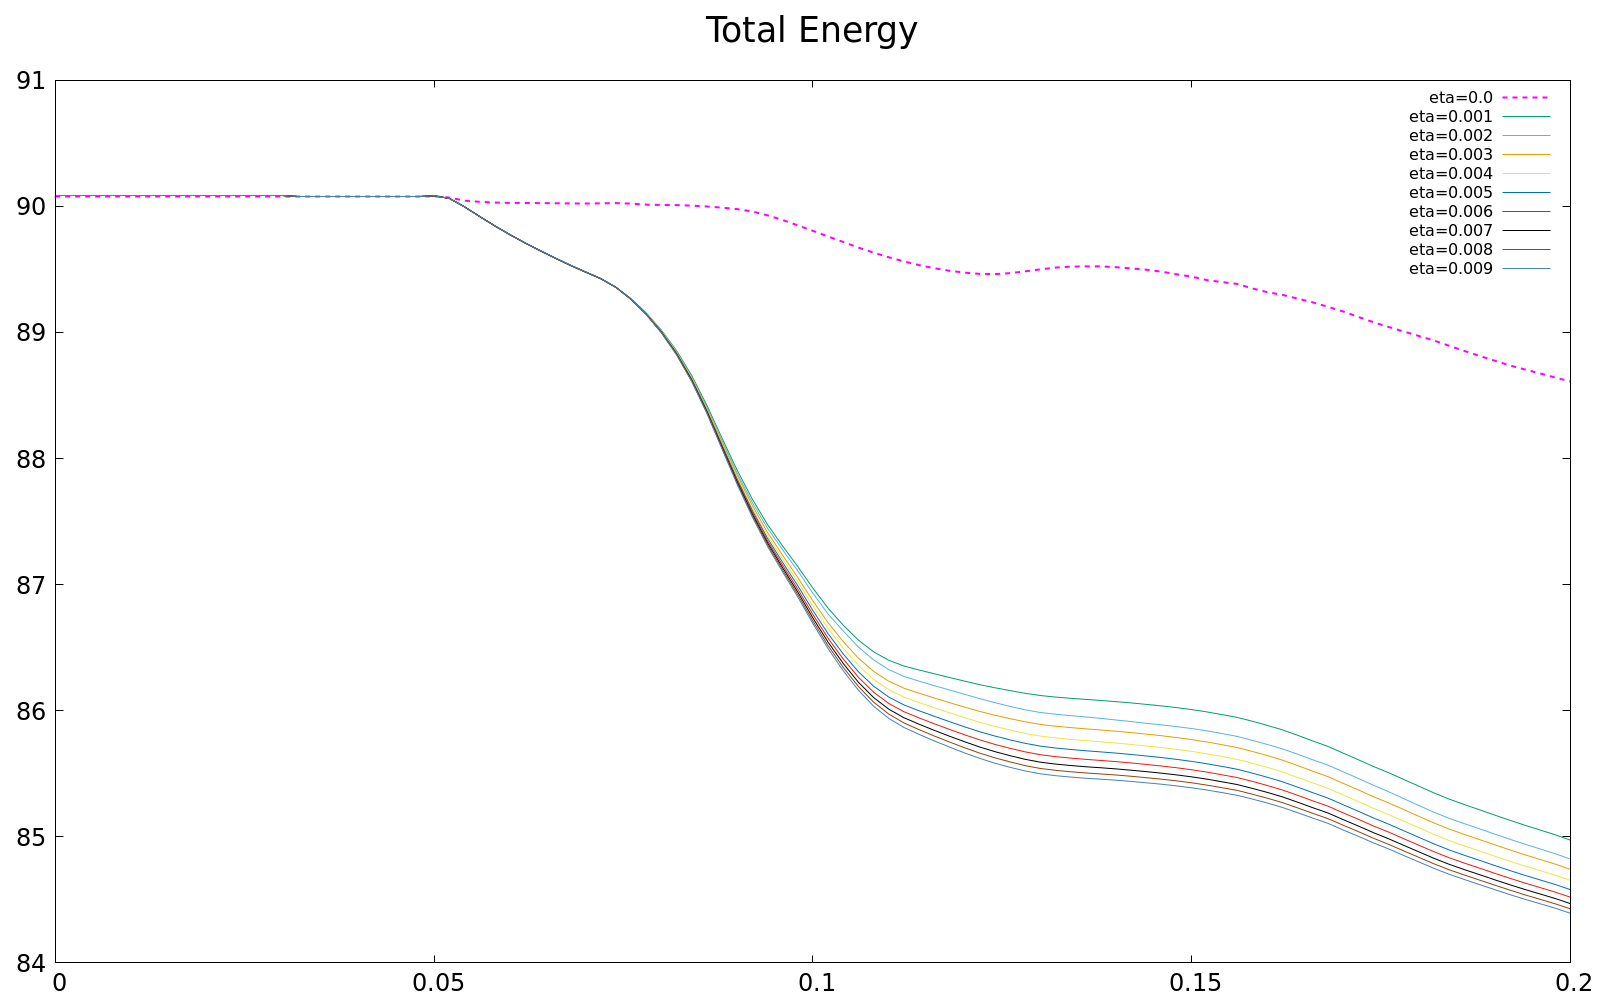
\includegraphics[width=1\linewidth]{TotalEnergy.png}
	\caption[Total energy curves]{This figure illustrates the temporal evolution of plasma total energy in the cylindrical equilibrium test, showing downward trends over time. As $\eta_w$ increases, the energy decreases further. The decline appears exponential, with diminishing energy reductions as $\eta_w$ increases.}
	\label{fig:totalEnergy}
\end{figure}



\section{Tokamak-shaped Application}
In earlier sections, the boundary conditions are validated and solvers with cylindrical equilibrium test. In this chapter, we apply this test in a container that more closely resembles a tokamak vessel. We build up a chamber similar to tokamak vessel in Ferraro \textit{et al.} \cite{ferraro2016multi}. We use tungsten as the vessel wall material. Hence, the resistivity is $5.6 \times 10^{-8} \, \Omega \cdot \text{m}$. The whole simulation is conducted under numerical domain of $[0.2,3.3]\times[-2.5,2.5]$ with $310\times500$ resolution. We extend the simulation to $t_{stop}=0.8$. 

The results are demonstrated in Figure \ref{fig:tokamak_application_inchapter9}. This simulation in the tokamak-shaped vessel provides valuable insights into the behavior of plasma under conditions that more closely resemble practical applications. As depicted in the figures, the simulation demonstrates the high-density plasma core impacting the tokamak wall. Upon impact, the plasma is observed to split and disperse along the wall. Unlike the cylindrical equilibrium test in the previous section, here, due to the very low resistivity of tungsten, the impact on the magnetic field when the wall is struck is hardly noticeable. It is also difficult to observe any significant plasma-wall interaction when the plasma moves along the boundary. After the initial impact, the more noticeable magnetic field fast magneto-acoustic waves are generated and propagate through the plasma. The figures show these waves spreading out from the impact region and interacting with other waves and structures within the vessel. They collide and interfere in the lower part of the vessel, which suggests the presence of non-linear wave interactions in the end of the simulation.


\begin{figure}[htbp]
	\centering
	
	\vspace{-5mm}
	% Row 1
	\hspace{-6mm}
	\begin{subfigure}{0.26\textwidth}
		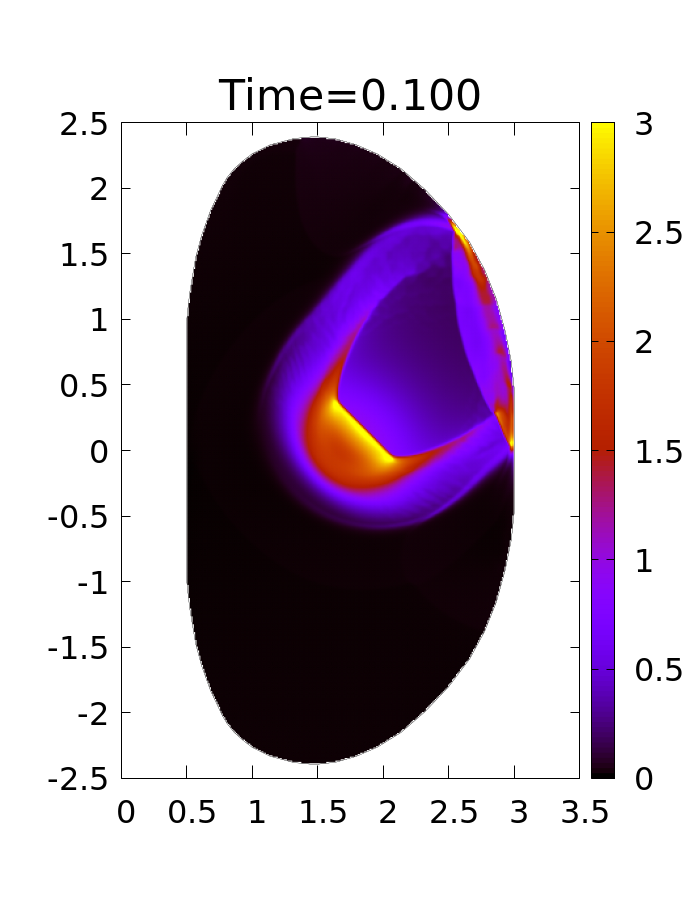
\includegraphics[width=\linewidth]{tokamak_Density_050.png}
	\end{subfigure}
	\hspace{-4mm} % Negative horizontal space
	\begin{subfigure}{0.26\textwidth}
		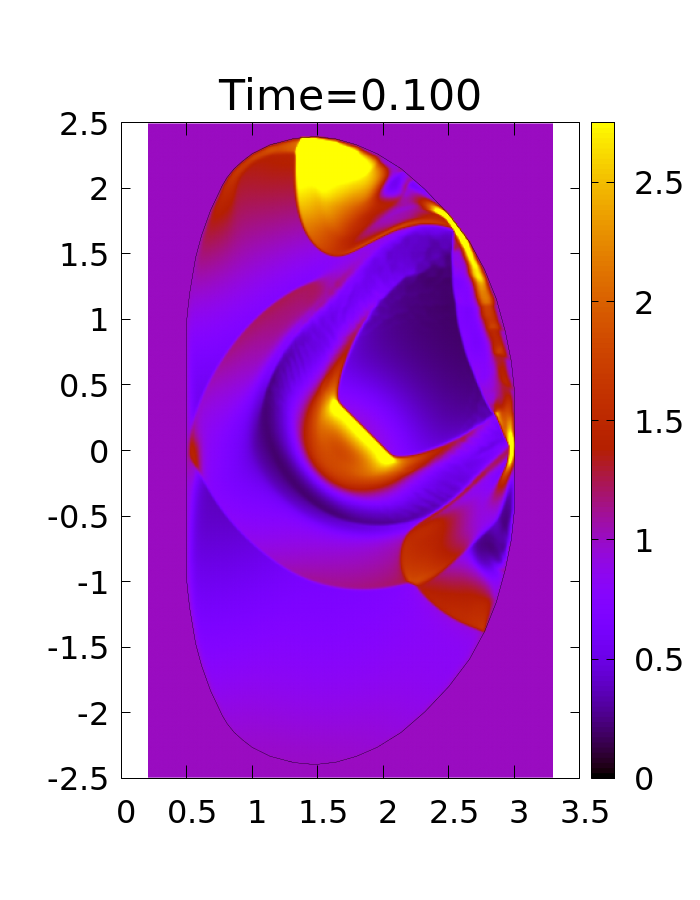
\includegraphics[width=\linewidth]{tokamak_Bz_050.png}
	\end{subfigure}
	\hspace{2mm} % Negative horizontal space
	\begin{subfigure}{0.26\textwidth}
		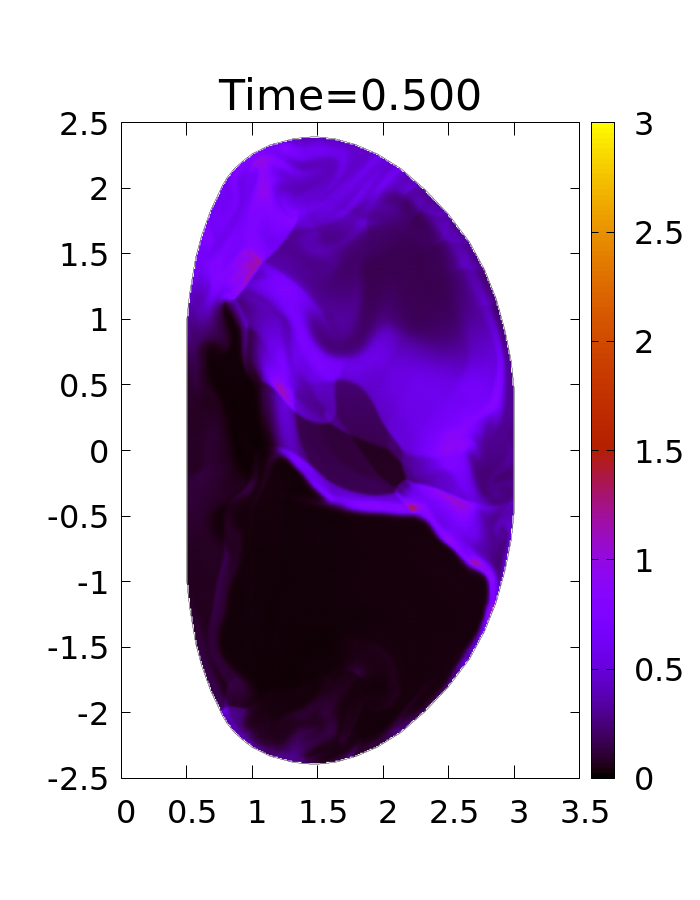
\includegraphics[width=\linewidth]{tokamak_Density_250.png}
	\end{subfigure}
	\hspace{-4mm} % Negative horizontal space
	\begin{subfigure}{0.26\textwidth}
		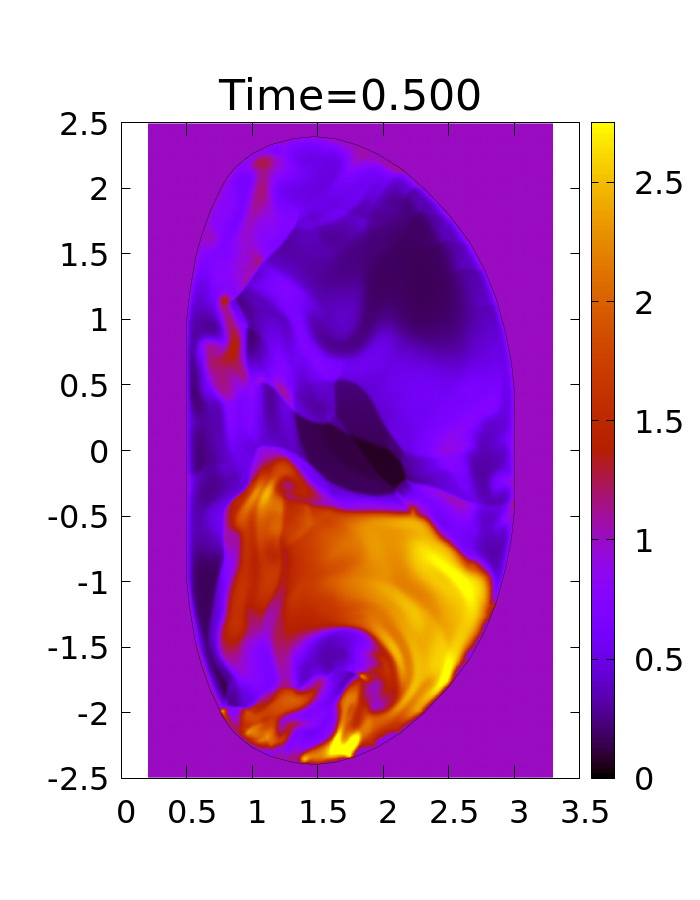
\includegraphics[width=\linewidth]{tokamak_Bz_250.png}
	\end{subfigure}
	\hspace{-6mm}
	
	\vspace{-6mm} % Negative vertical space
	
	% Row 2
	\hspace{-6mm}
	\begin{subfigure}{0.26\textwidth}
		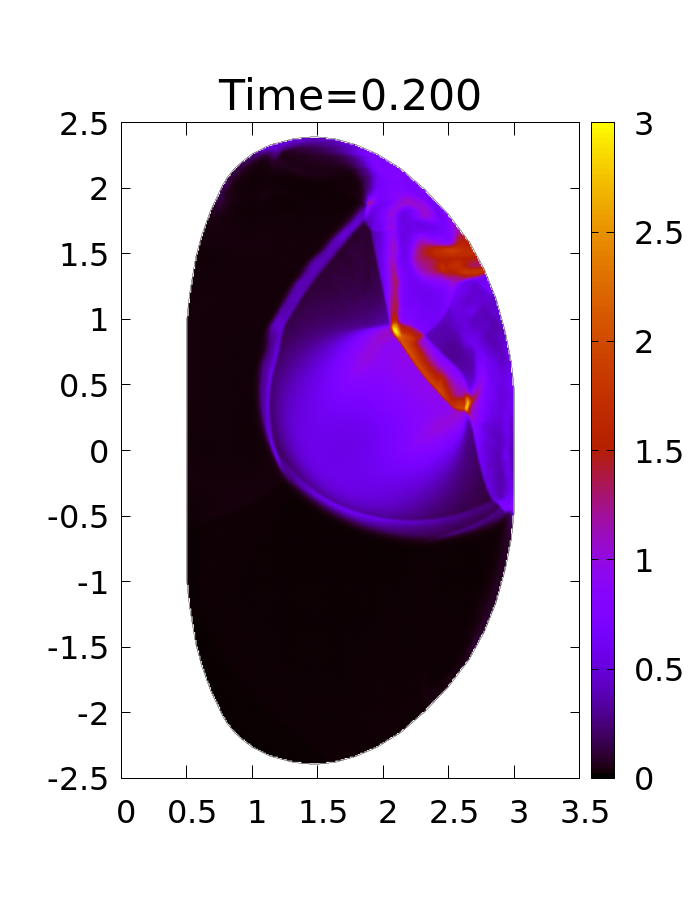
\includegraphics[width=\linewidth]{tokamak_Density_100.png}
	\end{subfigure}
	\hspace{-4mm} % Repeat negative space adjustments for each subfigure
	\begin{subfigure}{0.26\textwidth}
		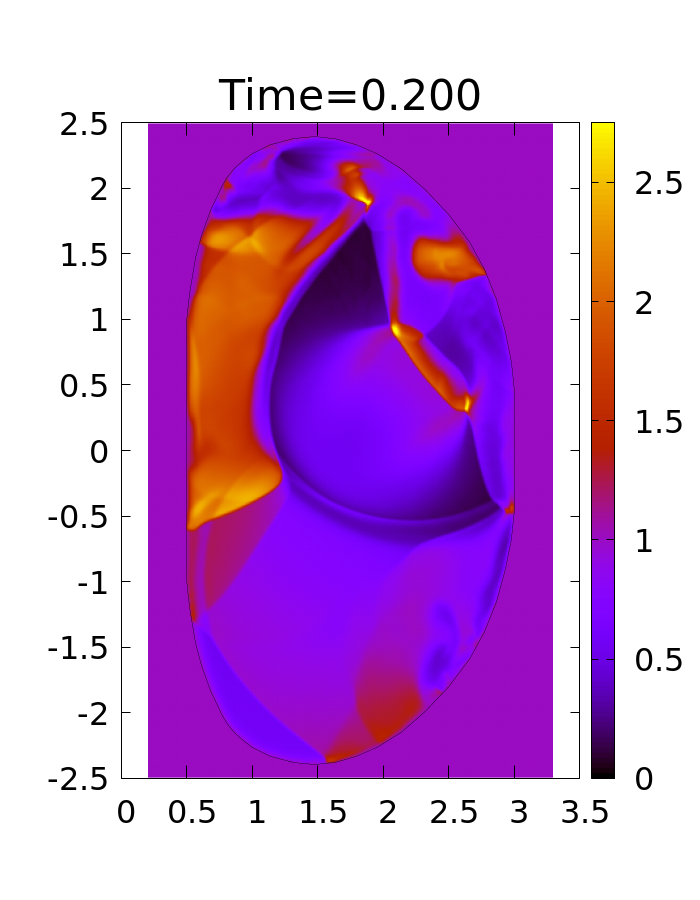
\includegraphics[width=\linewidth]{tokamak_Bz_100.png}
	\end{subfigure}
	\hspace{2mm} % Repeat negative space adjustments for each subfigure
	\begin{subfigure}{0.26\textwidth}
		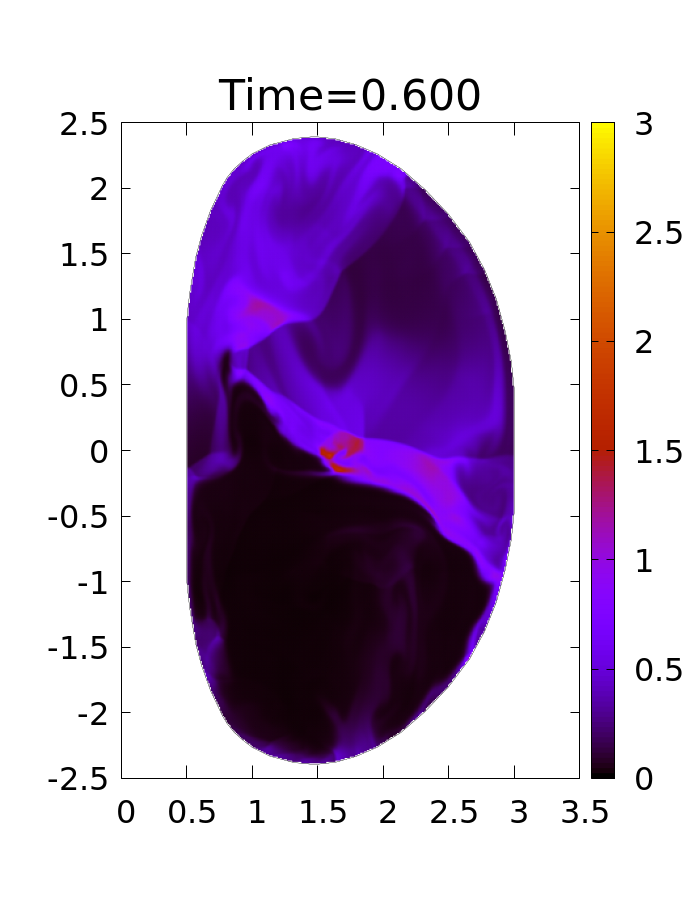
\includegraphics[width=\linewidth]{tokamak_Density_300.png}
	\end{subfigure}
	\hspace{-4mm} % Repeat negative space adjustments for each subfigure
	\begin{subfigure}{0.26\textwidth}
		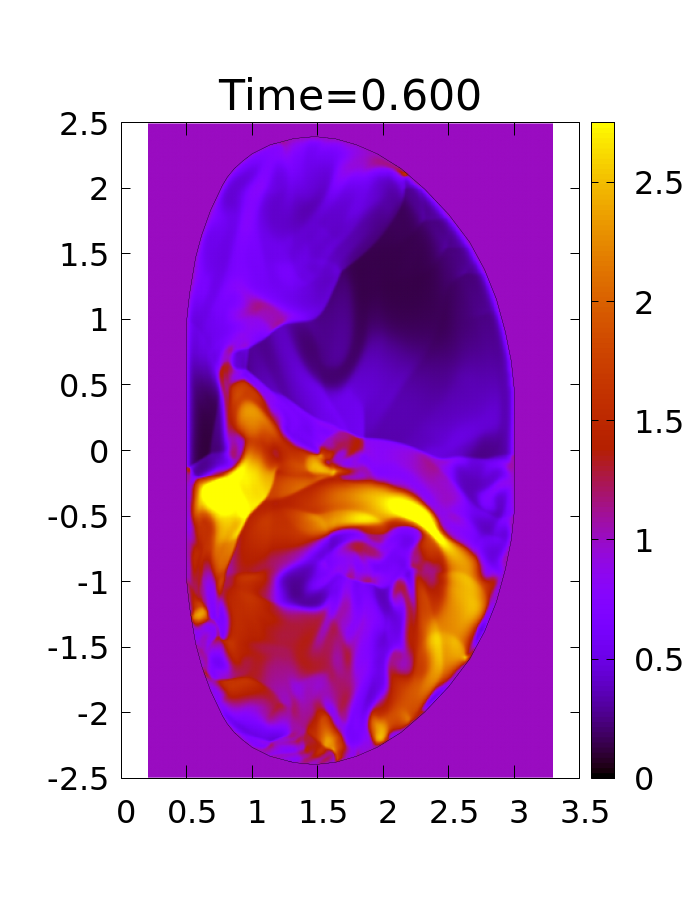
\includegraphics[width=\linewidth]{tokamak_Bz_300.png}
	\end{subfigure}
	\hspace{-5mm}
	
	\vspace{-6mm} % Negative vertical space
	
	% Row 3
	\hspace{-6mm}
	\begin{subfigure}{0.26\textwidth}
		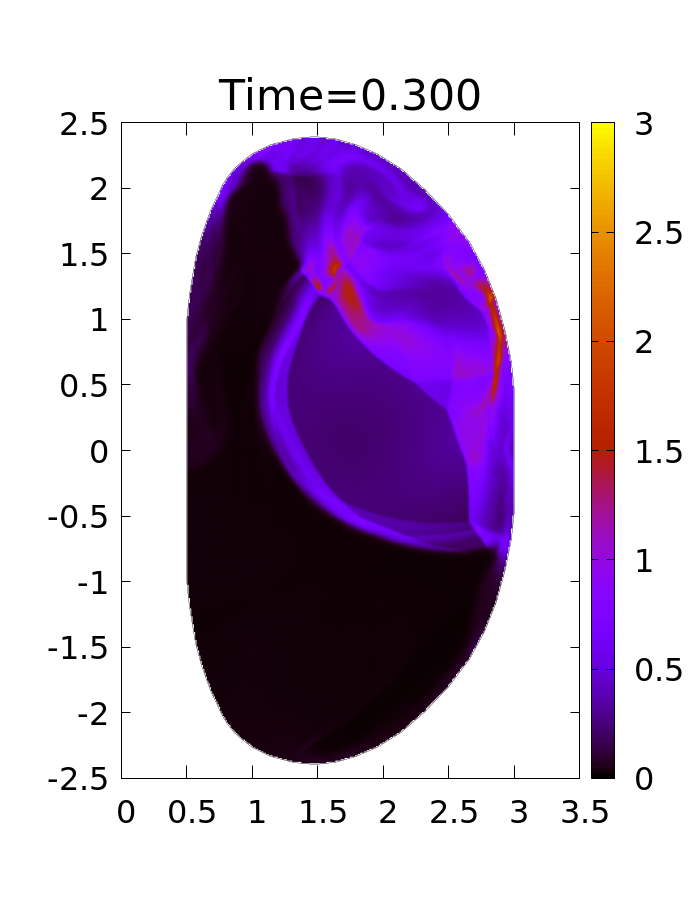
\includegraphics[width=\linewidth]{tokamak_Density_150.png}
	\end{subfigure}
	\hspace{-4mm} % Repeat negative space adjustments for each subfigure
	\begin{subfigure}{0.26\textwidth}
		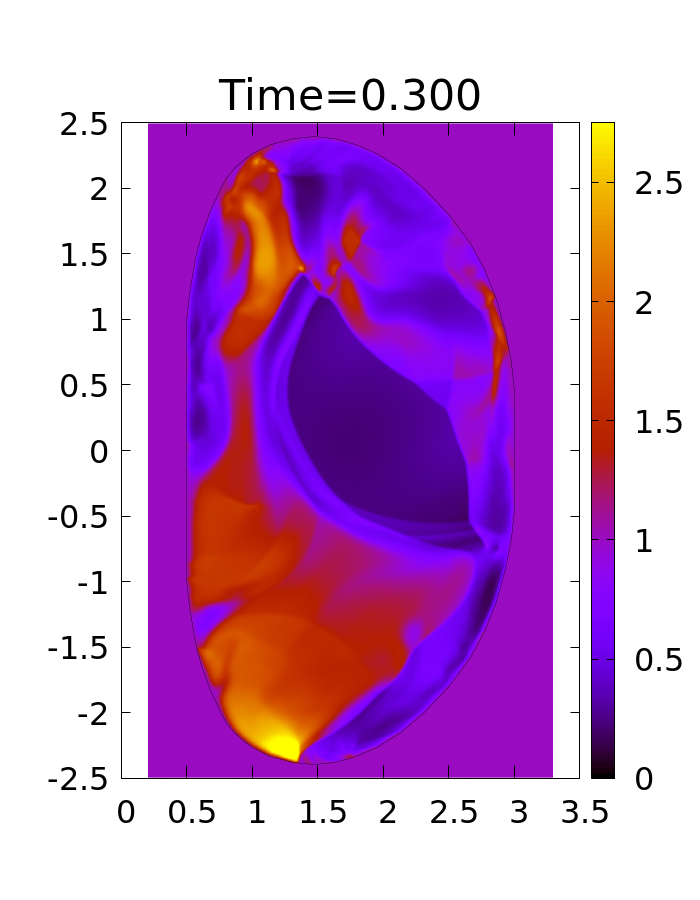
\includegraphics[width=\linewidth]{tokamak_Bz_150.png}
	\end{subfigure}
	\hspace{2mm} % Repeat negative space adjustments for each subfigure
	\begin{subfigure}{0.26\textwidth}
		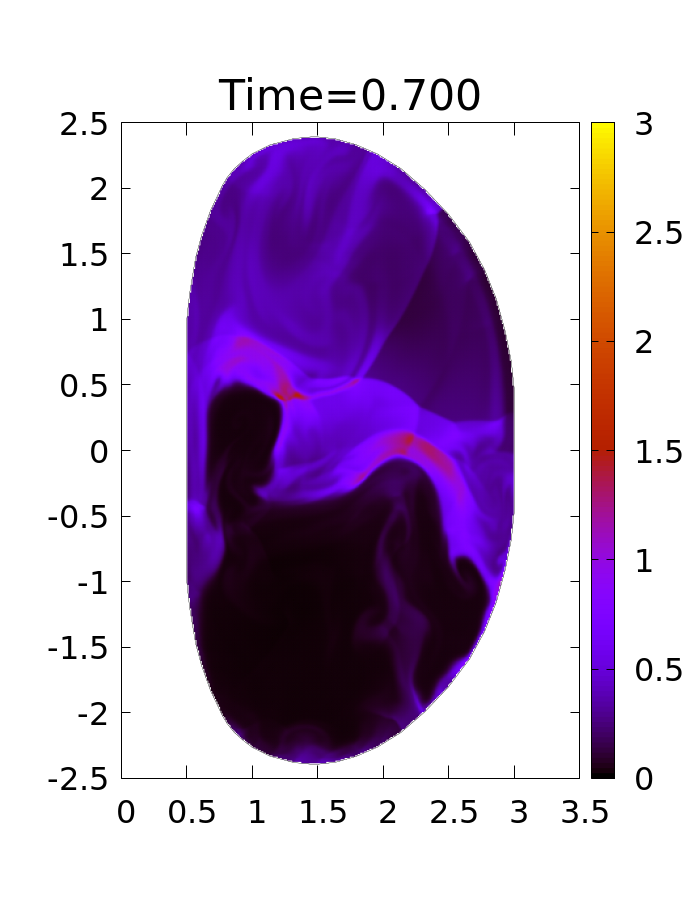
\includegraphics[width=\linewidth]{tokamak_Density_350.png}
	\end{subfigure}
	\hspace{-4mm} % Repeat negative space adjustments for each subfigure
	\begin{subfigure}{0.26\textwidth}
		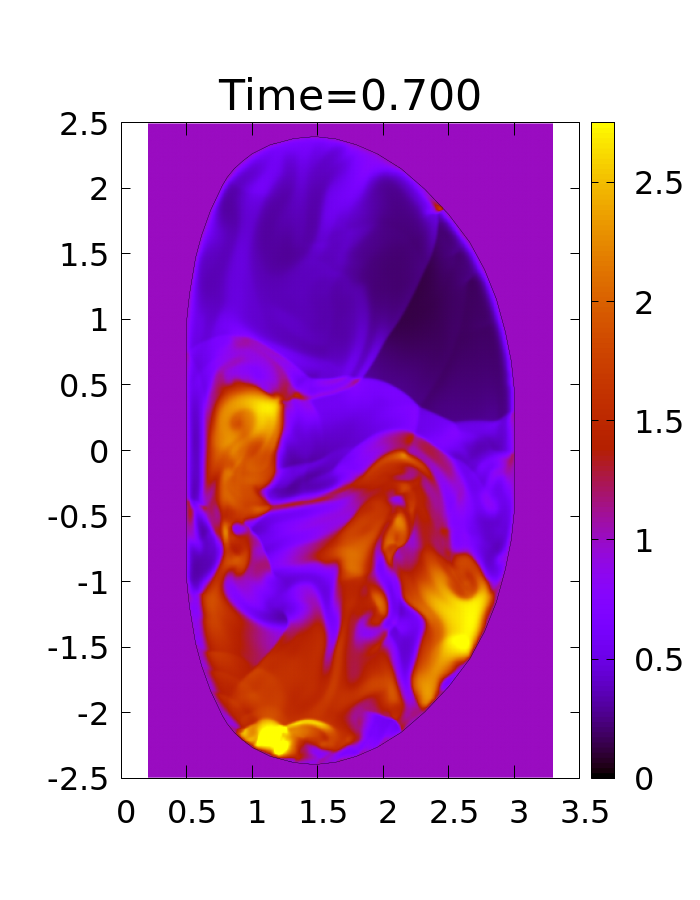
\includegraphics[width=\linewidth]{tokamak_Bz_350.png}
	\end{subfigure}
	\hspace{-6mm}
	
	\vspace{-6mm} % Negative vertical space
	
	% Row 4 
	\hspace{-6mm}
	\begin{subfigure}{0.26\textwidth}
		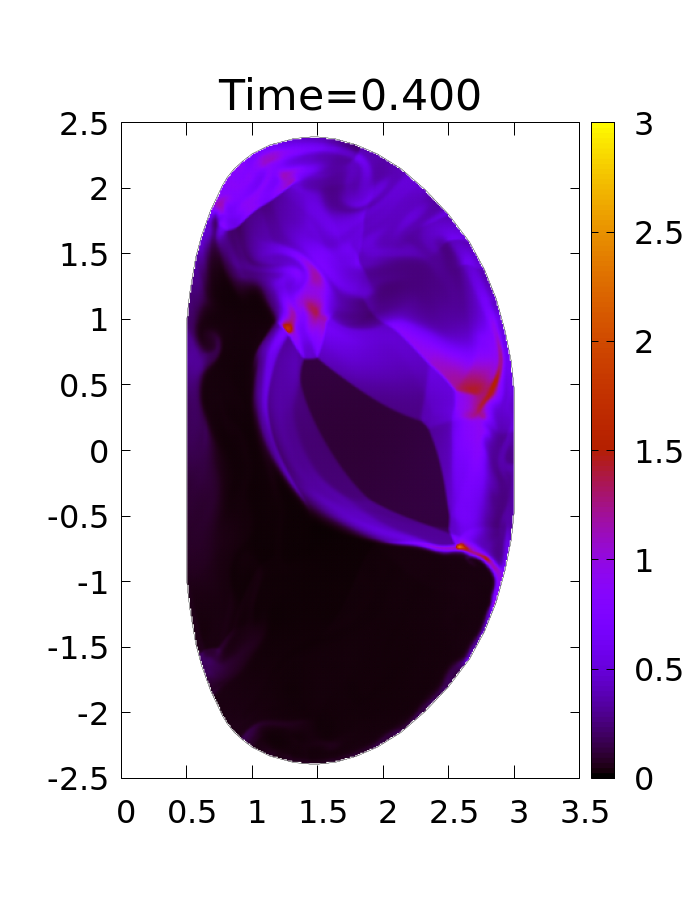
\includegraphics[width=\linewidth]{tokamak_Density_200.png}
		\caption*{Density}
	\end{subfigure}
	\hspace{-4mm} % Repeat negative space adjustments for each subfigure
	\begin{subfigure}{0.26\textwidth}
		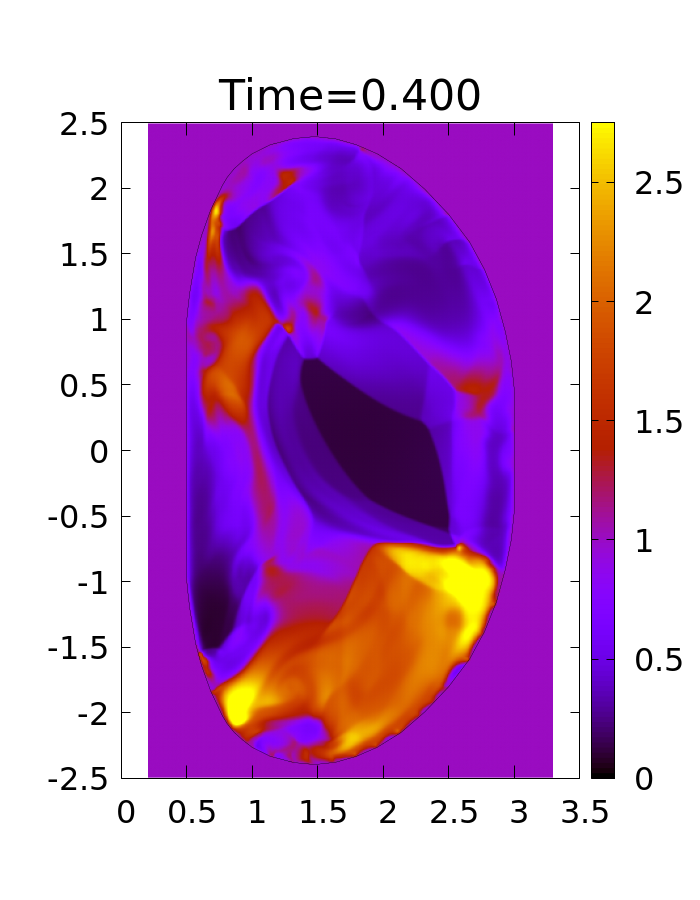
\includegraphics[width=\linewidth]{tokamak_Bz_200.png}
		\caption*{$B_z$}
	\end{subfigure}
	\hspace{2mm} % Repeat negative space adjustments for each subfigure
	\begin{subfigure}{0.26\textwidth}
		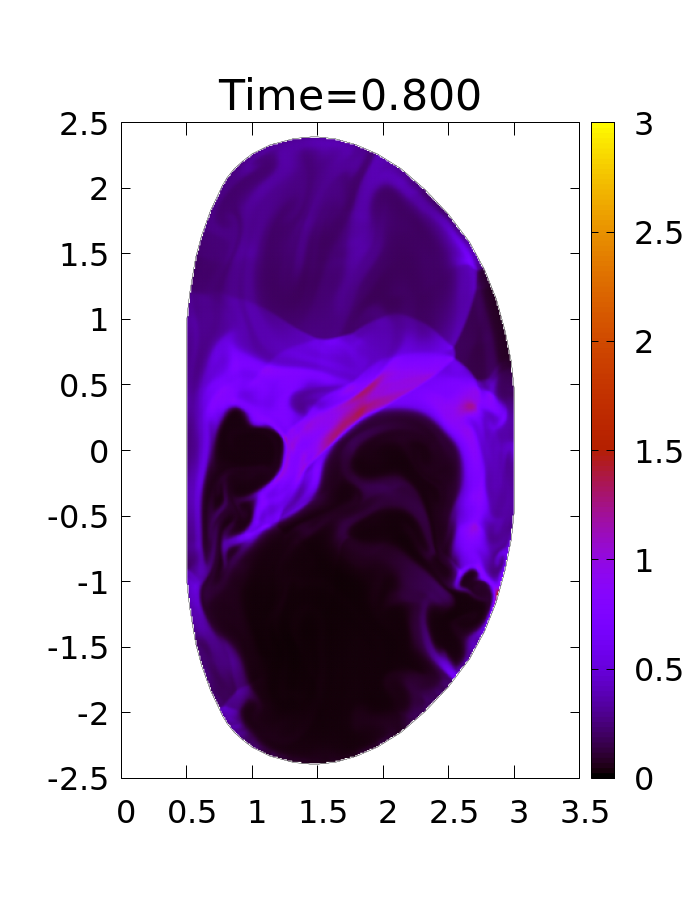
\includegraphics[width=\linewidth]{tokamak_Density_400.png}
		\caption*{Density}
	\end{subfigure}
	\hspace{-4mm} % Repeat negative space adjustments for each subfigure
	\begin{subfigure}{0.26\textwidth}
		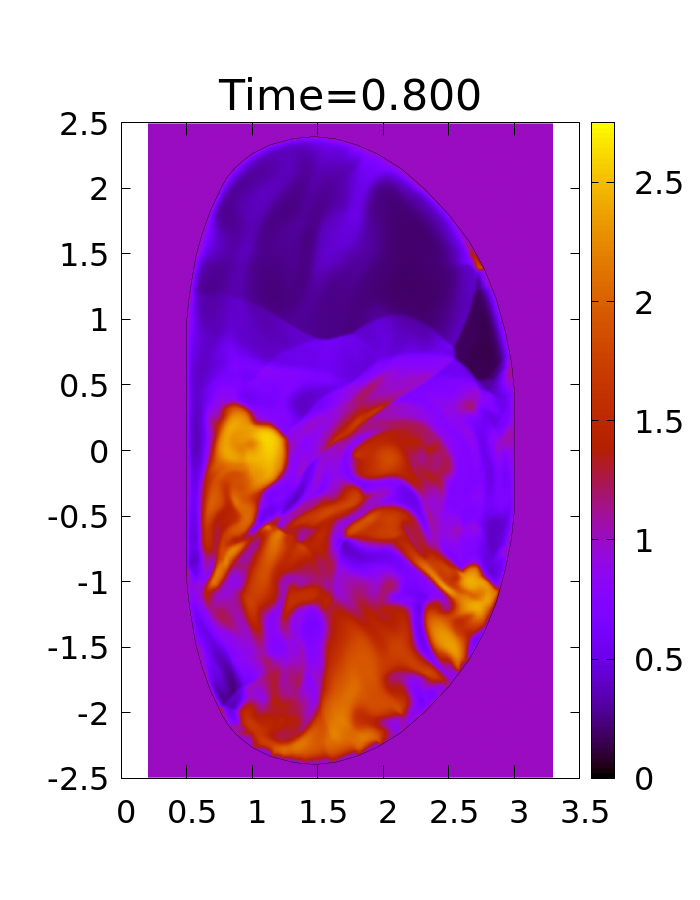
\includegraphics[width=\linewidth]{tokamak_Bz_400.png}
		\caption*{$B_z$}
	\end{subfigure}
	\hspace{-6mm}
	
	\vspace{1mm} % Negative vertical space
	
	\caption[Tokamak Application]{Simulation of the cylindrical equilibrium test in a tokamak-shaped vessel. The wall is assumed to be made of tungsten, with a resistivity of $5.6 \times 10^{-8} \, \Omega \cdot \text{m}$.}
	\label{fig:tokamak_application_inchapter9}
\end{figure}


  
